% !TeX spellcheck = ru_RU
% !TEX root = vkr.tex

В среде ОС Embox были запущены некоторые приложения, осуществляющие системные вызовы Linux и скомпилированные для исполнения в среде ОС GNU/Linux.

Стоит отметить, что на момент написания данной работы в ОС Embox отсутствует возможность использовать механизм \textit{разделяемых библиотек} (англ. shared libraries). Это означает, что участвующие в апробации двоичные файлы должны быть скомпонованы полностью статически (не использовать механизм разделяемых библиотек). Даже простые программные инструменты в ОС GNU/Linux, такие как \texttt{echo}, напротив, компонуются динамически относительно библиотеки GLIBC\,\footnote{Например, даже такие функции как \texttt{write} и \texttt{read}, которые выглядят как <<прямые>> системные вызовы Linux, на самом деле являются функциями-обёртками, предоставляемыми библиотекой GLIBC.}. Более того, на практике очень сложно скомпоновать полностью статическую программу, если она использует GLIBC~--- библиотека не проектировалась для этого, попытки статической компоновки приведут к целому ряду проблем~\cite{glibc}. В качестве обходного пути можно попробовать использовать вместо GLIBC более подходящую для статической компоновки библиотеку, например библиотеку uClibc~\cite{uclibc}. Однако, автором был выбран иной путь~--- для ряда стандартных программных инструментов GNU/Linux были реализованы упрощённые аналоги, не использующие стандартную библиотеку Си. Для осуществления системного вызова Linux в этих программах используется аналог предоставляемой библиотекой GLIBC функции \texttt{syscall} (вызывает инструкцию \texttt{INT0x80} с заданными номером и аргументами системного вызова), на основе которого реализованы другие стандартные функции.

В первую очередь работоспособность модуля слоя двоичной совместимости была протестирована при помощи программы \texttt{linux\_echo}, выводящей передаваемый ей параметр в стандартный поток вывода (терминал). После компиляции программа работает как в среде GNU/Linux (рис.\,\ref{fig:linux_echo}), так и в среде ОС Embox (рис.\,\ref{fig:embox_echo}).

\begin{figure}[H]
\center{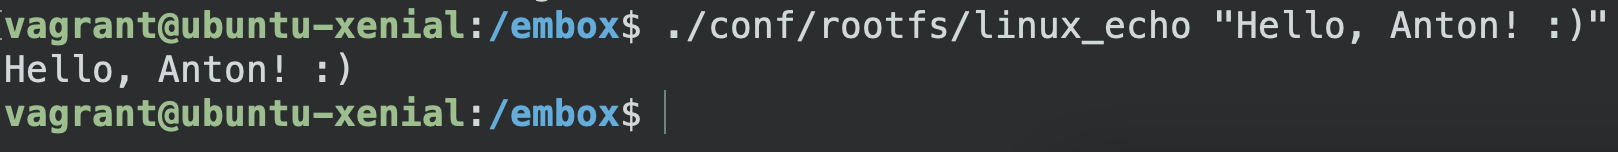
\includegraphics[scale=0.55]{pictures/linux_echo.png}}
\caption{Исполнение \texttt{linux\_echo} в ОС Ubuntu}
\label{fig:linux_echo}
\end{figure}

\begin{figure}[H]
\center{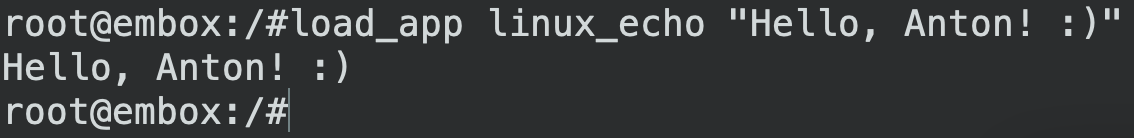
\includegraphics[scale=0.65]{pictures/embox_echo.png}}
\caption{Исполнение \texttt{linux\_echo} в ОС Embox}
\label{fig:embox_echo}
\end{figure}

Также, была продемонстрирована работа с \texttt{procfs}~--- специальной файловой системой Linux, предназначенной для получения некоторой служебной информации от ядра Linux. Эта файловая система реализуется в коде ядра Linux. Она не специфицирована, поэтому в ОС Embox может либо отсутствовать, либо иметь произвольную реализацию. Данный пример показывает, что программы GNU/Linux, которые зависят от подобных элементов ядра Linux, могут работать без необходимости реализации этих элементов в ОС Embox в том виде, в каком они существуют в ядре Linux (один из плюсов метода паравиртуализации).

Сначала в средах GNU/Linux (рис.\,\ref{fig:linux_ls}) и ОС Embox (рис.\,\ref{fig:embox_ls_root}, рис.\,\ref{fig:embox_ls_proc}) была запущена программа \texttt{linux\_ls}, выводящая содержимое заданного каталога. Затем, при помощи программы \texttt{linux\_cat} в обеих средах были прочитаны данные из некоторых файлов, предоставляемых файловой системой \texttt{procfs} (рис.\,\ref{fig:linux_cat}, рис.\,\ref{fig:embox_cat_devices}, рис.\,\ref{fig:embox_cat_stat}, рис.\,\ref{fig:embox_cat_slabinfo}).

\begin{figure}[H]
\center{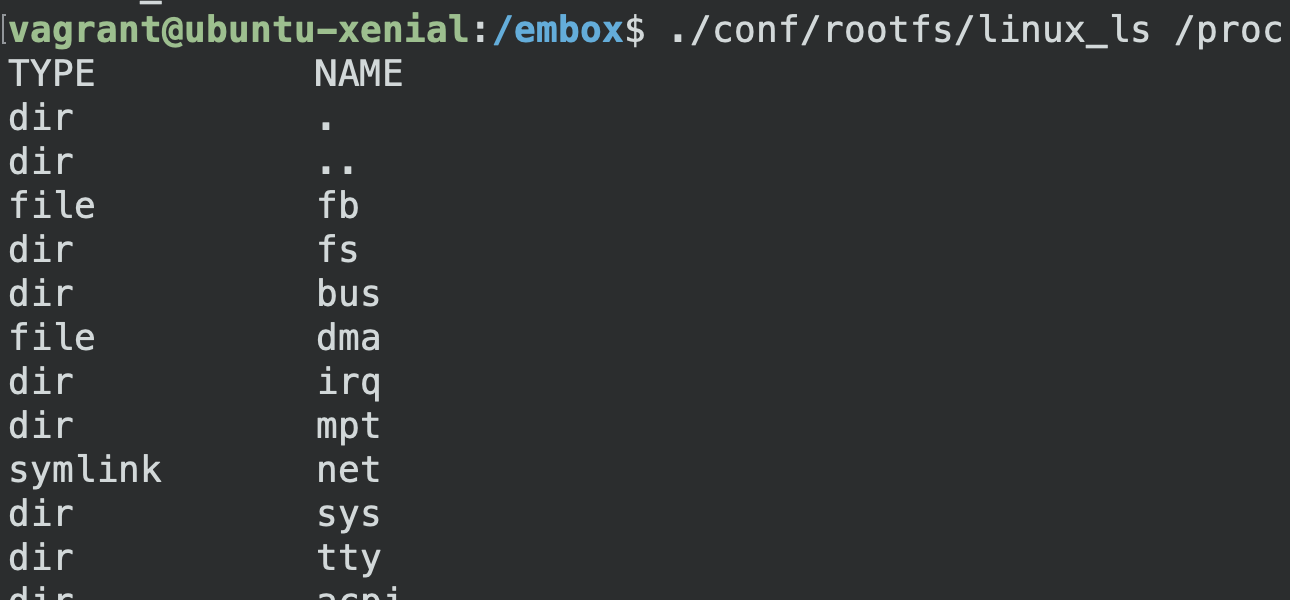
\includegraphics[scale=0.45]{pictures/linux_ls.png}}
\caption{Исполнение \texttt{linux\_ls} (каталог \texttt{/proc}) в ОС Ubuntu}
\label{fig:linux_ls}
\end{figure}

\begin{figure}[H]
\center{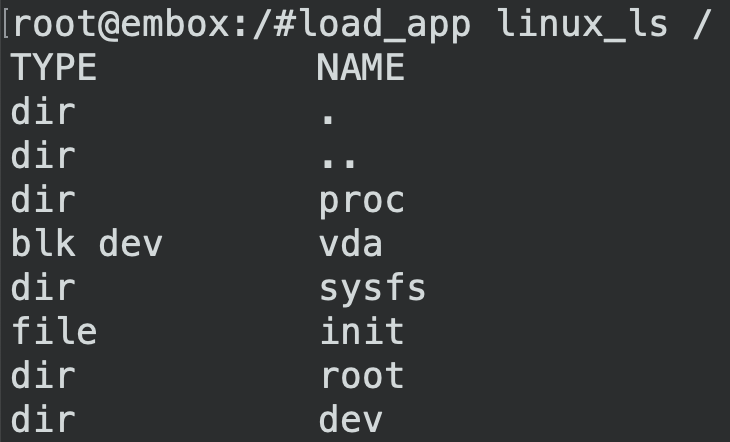
\includegraphics[scale=0.45]{pictures/embox_ls_root.png}}
\caption{Исполнение \texttt{linux\_ls} (корневой каталог) в ОС Embox}
\label{fig:embox_ls_root}
\end{figure}

\begin{figure}[H]
\center{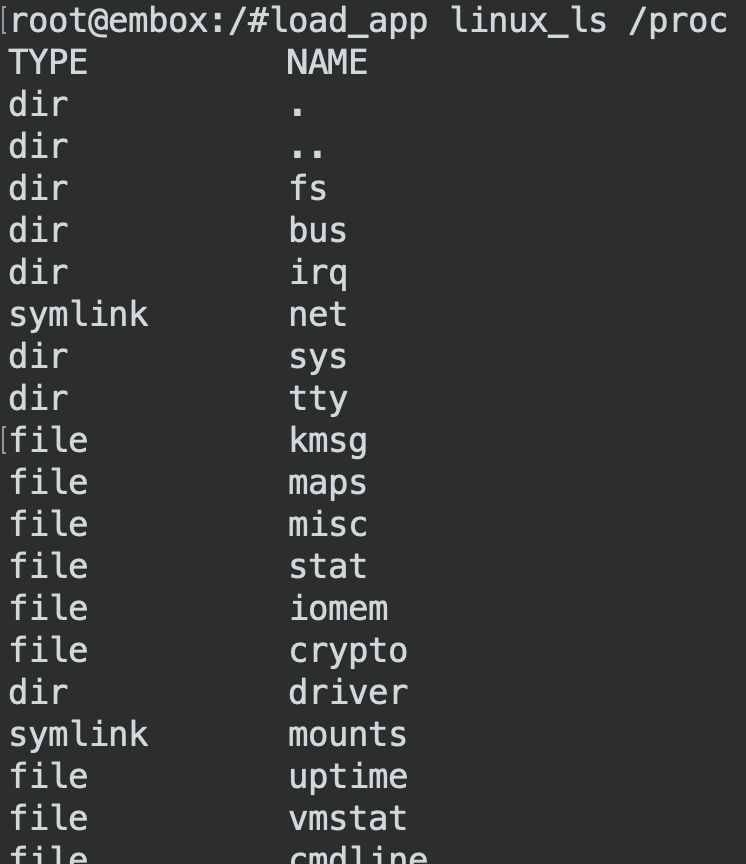
\includegraphics[scale=0.35]{pictures/embox_ls_proc.png}}
\caption{Исполнение \texttt{linux\_ls} (каталог \texttt{/proc}) в ОС Embox}
\label{fig:embox_ls_proc}
\end{figure}

\begin{figure}[H]
\center{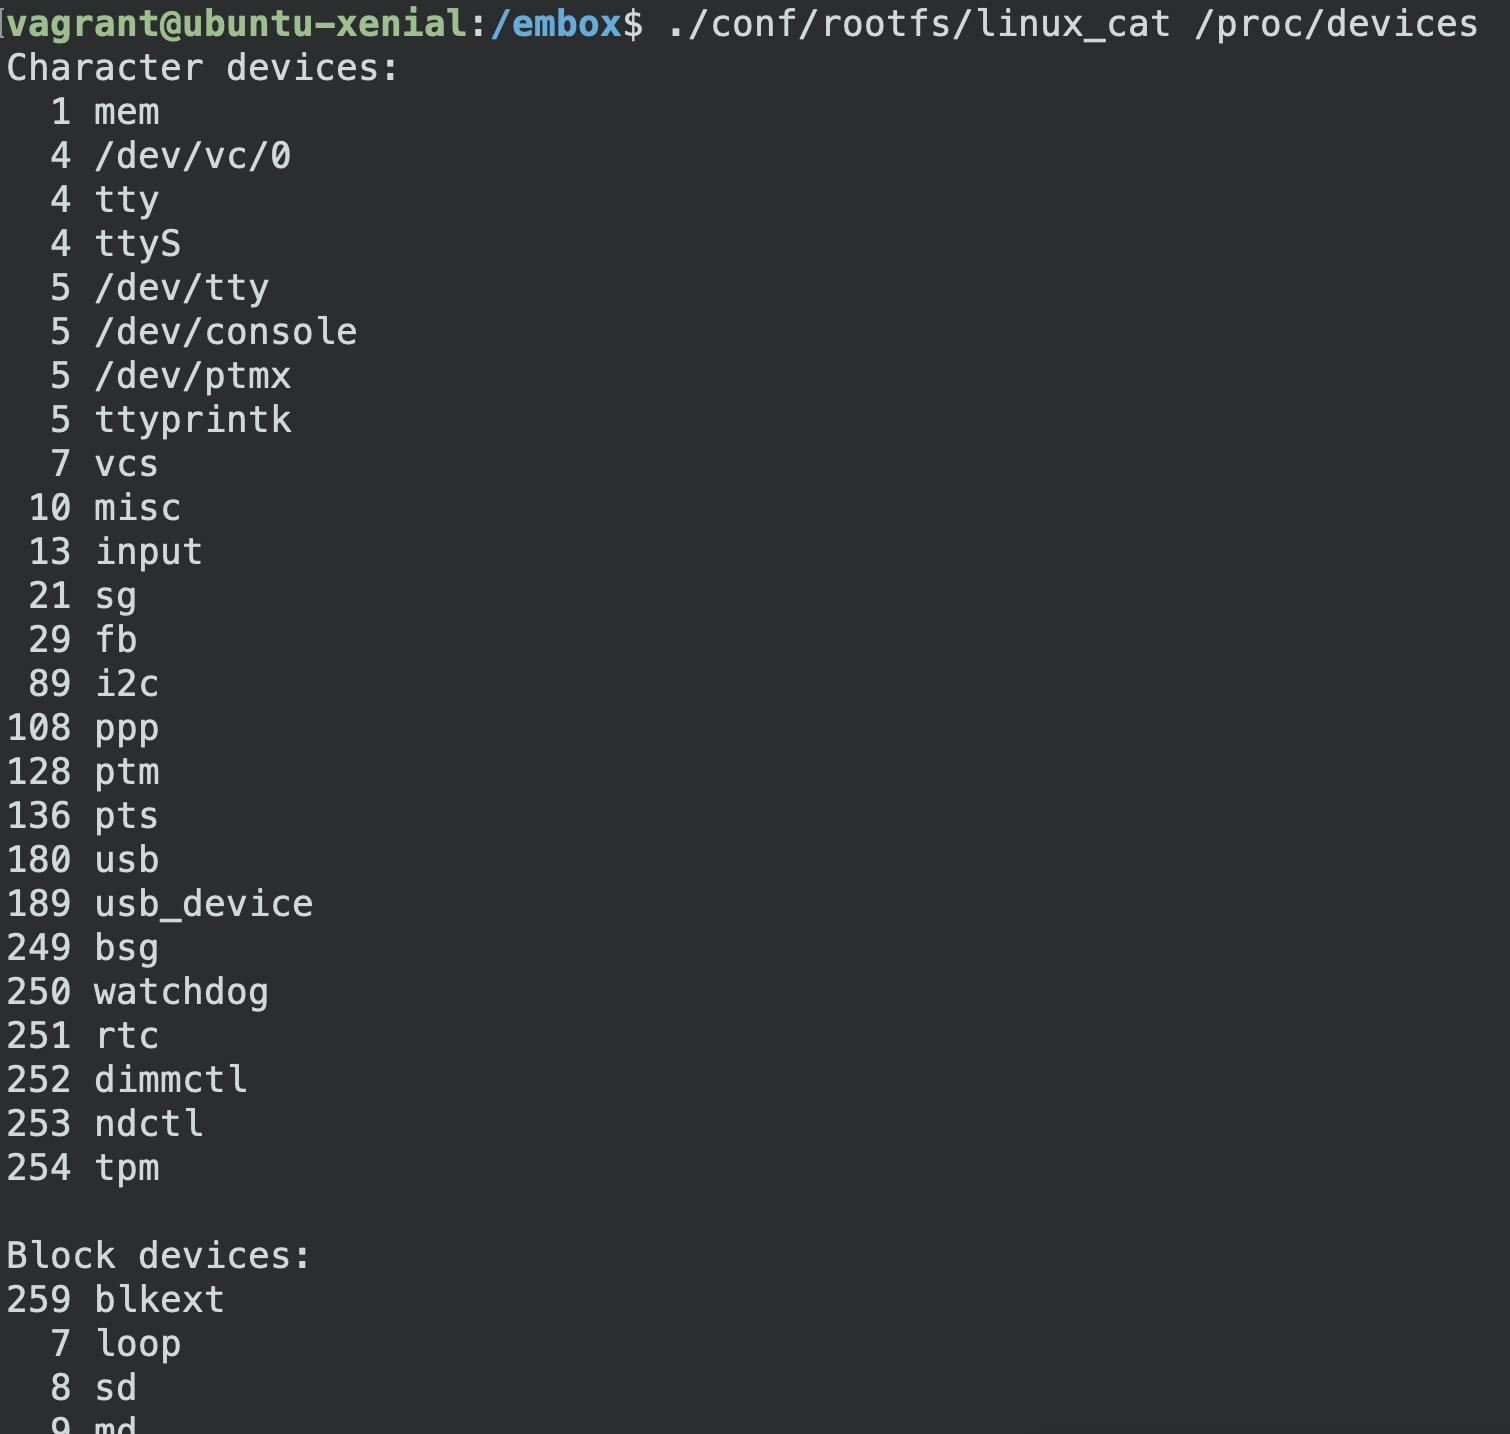
\includegraphics[scale=0.25]{pictures/linux_cat.png}}
\caption{Исполнение \texttt{linux\_cat} (файл \texttt{/proc/devices}) в ОС Ubuntu}
\label{fig:linux_cat}
\end{figure}

\begin{figure}[H]
\center{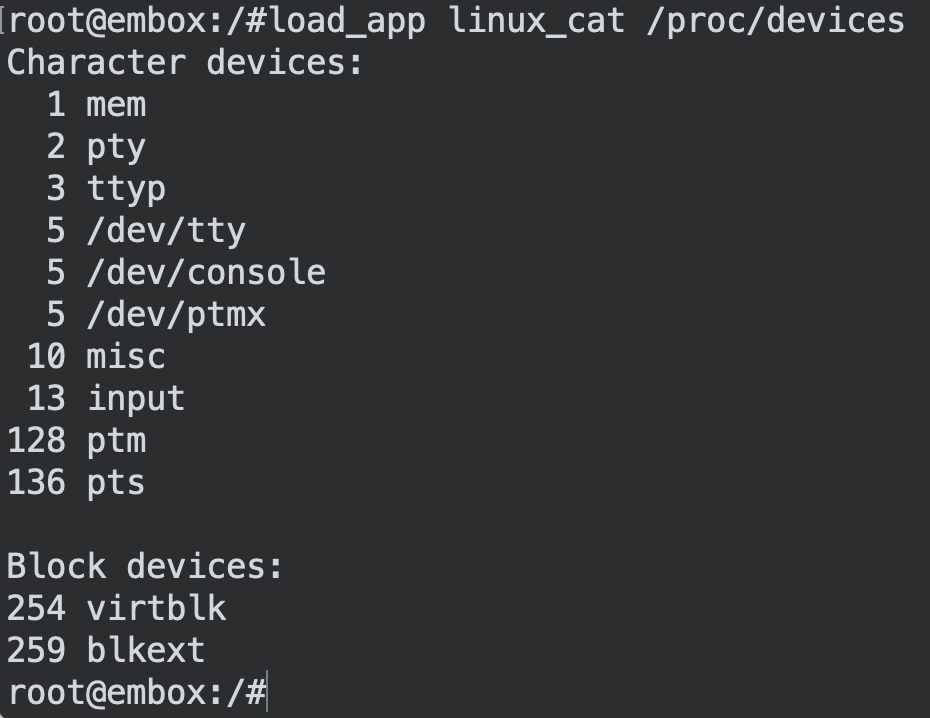
\includegraphics[scale=0.45]{pictures/embox_cat_devices.png}}
\caption{Исполнение \texttt{linux\_cat} (файл \texttt{/proc/devices}) в ОС Embox}
\label{fig:embox_cat_devices}
\end{figure}

\begin{figure}[H]
\center{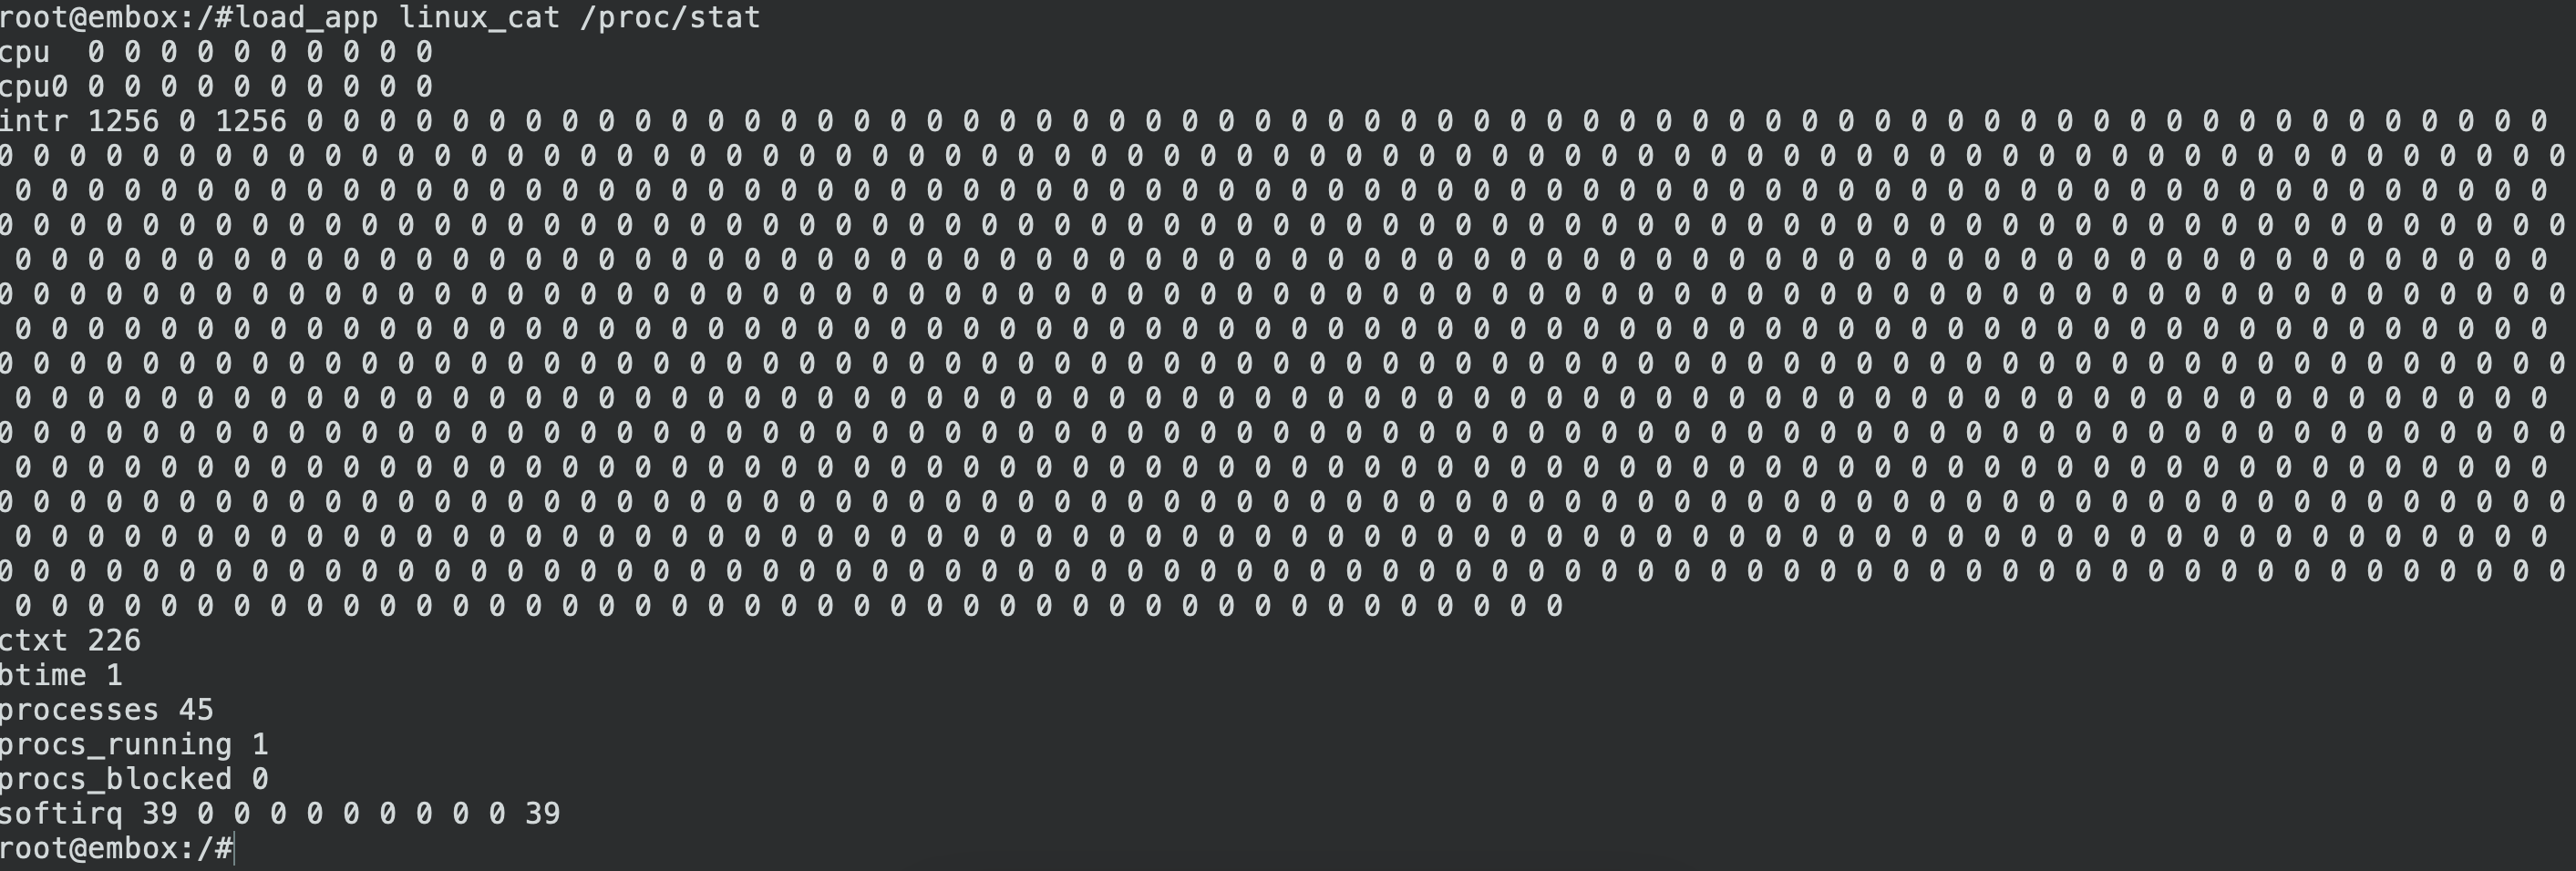
\includegraphics[scale=0.25]{pictures/embox_cat_stat.png}}
\caption{Исполнение \texttt{linux\_cat} (файл \texttt{/proc/stat}) в ОС Embox}
\label{fig:embox_cat_stat}
\end{figure}

\begin{figure}[H]
\center{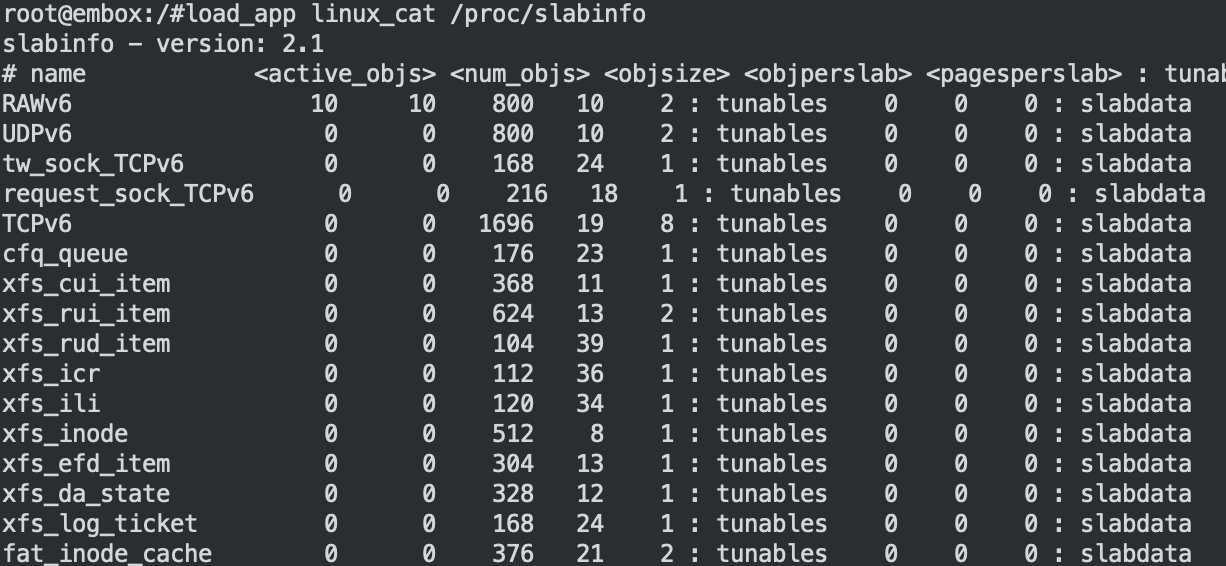
\includegraphics[scale=0.45]{pictures/embox_cat_slabinfo.png}}
\caption{Исполнение \texttt{linux\_cat} (файл \texttt{/proc/slabinfo}) в среде Embox}
\label{fig:embox_cat_slabinfo}
\end{figure}

Такая демонстрация задействует всю цепочку компонентов слоя двоичной совместимости. В ОС Embox есть два разных окружения~--- одно является обычным окружением Embox, другое предоставляется реализованной подсистемой. В среде Embox запускаются приложения, совершающие системные вызовы Linux. Паравиртуализируемое ядро Linux (библиотека LKL) выполняет обработку этих системных вызовов. Виртуальное устройство внутри LKL успешно выводит текст на терминал Embox. Процессу ОС Embox доступно как обычное окружение Embox, так и окружение, предоставляемое подсистемой с ядром Linux.
